
\chapter{Numerical analysis}
It is interesting to perform a numerical analysis of the leading-twist NLO cross section presented so far. In order to do so, one needs to access the relevant PDFs and FFs that show up in the formulae. When it comes to unpolarized PDFs, we use the MSTW 2008 PDF set presented in \cite{Martin_2009}. For unpolarized fragmentation, we employ the DSS FF set \cite{de_Florian_2007}. In Fig.~\ref{fig:f1D1}, curves for $f_1(x)$ and $D_1(z)$ are presented, showcasing different flavors contributions.
\begin{figure}
    \centering
    \subfigure[]{\centering
                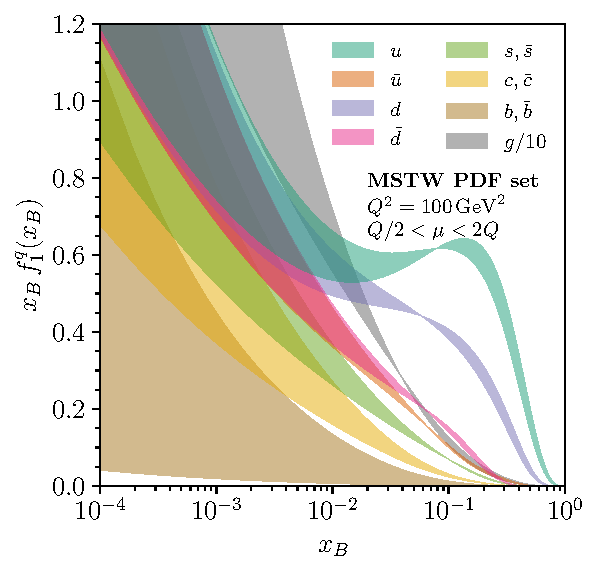
\includegraphics[width=0.45\linewidth]{fig/f1.pdf}
    }
    \hfill
        \subfigure[]{\centering
                    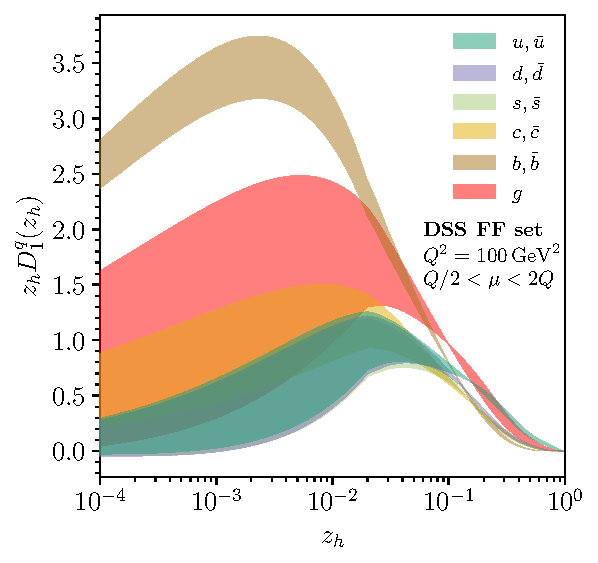
\includegraphics[width=0.45\linewidth]{fig/D1.pdf}
    }
    \caption{Leading-twist unpolarized $f_1$ PDF and $D_1$ FF as a function of $x_B$ and $z_h$, respectively. Different colors represent different flavors. The scale variation is supposed to give an idea on how much these distributions vary if evaluated at different scales.}
    \label{fig:f1D1}
\end{figure}
It is also interesting to study the leading-twist, unpolarized, triple differential cross section $\dd \sigma/\dd x_B \dd y \dd z_h$ at NLO. A plot of this cross section as a function of the different kinematical variables is shown in Fig.~\ref{fig:plotNLOUUU}. We observe sizable NLO corrections to the LO cross section, especially at the edges of the phase space of the three kinematical variables. This is a common feature of NLO corrections in QCD.
\begin{figure}
    \centering
    \subfigure[]{
    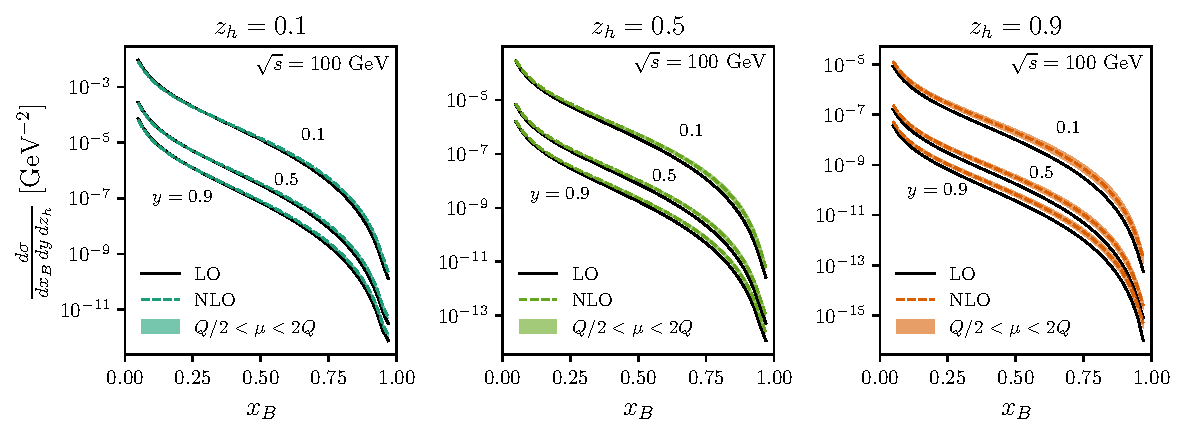
\includegraphics[width=0.92\textwidth]{fig/sigmaUUU_NLO(x).pdf}
    }
    \subfigure[]{
    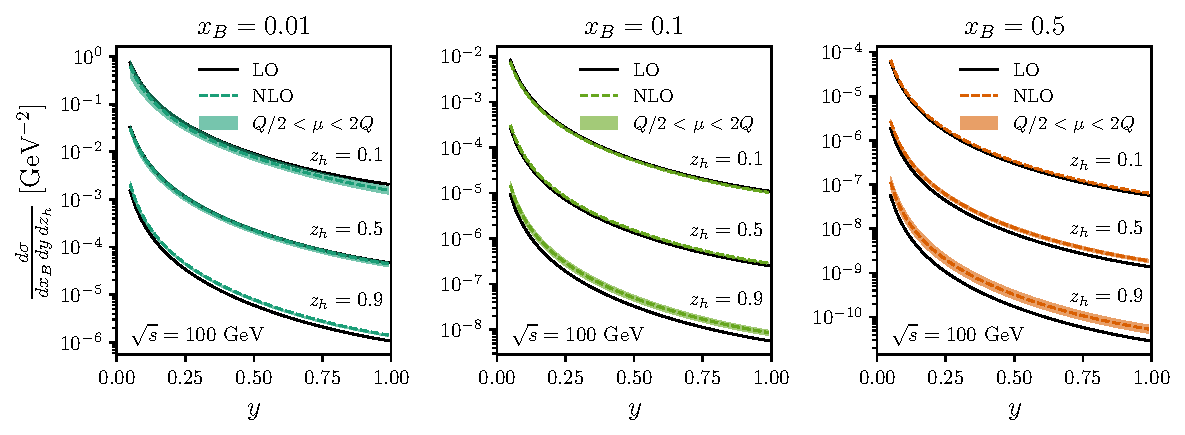
\includegraphics[width=0.92\textwidth]{fig/sigmaUUU_NLO(y).pdf}
    }
    \subfigure[]{
    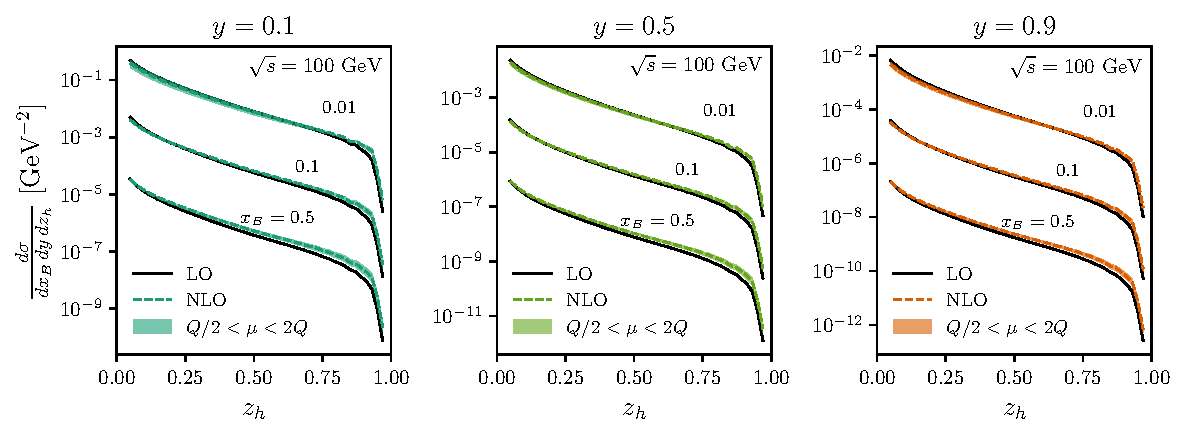
\includegraphics[width=0.92\textwidth]{fig/sigmaUUU_NLO(z).pdf}
    }
    \caption{Unpolarized leading-twist cross section at LO and NLO accuracy as a function of $x_B$ (panel a), $y$ (panel b) and $z_h$ (panel c).}
    \label{fig:plotNLOUUU}
\end{figure} 

Add pheno of transversity with jam3d. Add curves for asymmetry/polarized structure functions
%cherednikova van der veken parton densities in quantum chromodynamics free pdf

\clearpage

